\documentclass{article}
\usepackage[margin=1in]{geometry} 
\usepackage{amsmath,amsthm,amssymb,amsfonts, fancyhdr, color, comment, graphicx, environ}
\usepackage{xcolor}
\usepackage{mdframed}
\usepackage[shortlabels]{enumitem}
\usepackage{indentfirst}
\usepackage{hyperref}
\hypersetup{
    colorlinks=true,
    linkcolor=blue,
    filecolor=magenta,      
    urlcolor=blue,
}
\usepackage{pgfplots}
\pgfplotsset{width=10cm,compat=1.9}
\pgfplotsset{compat=1.17}
\usepackage{tikz}
\usepackage{caption}

\setlength{\parindent}{0pt}


%for headers 
\pagestyle{fancy}
\fancyhf{} % for header/footer

\lhead{Creel}
\rhead{ENV 795 - Nature as Capital}
\chead{\textbf{Natural Capital}}

\title{Week Four - Natural Capital and Sustainability}
\author{Andie Creel for Nature as Capital}
\date{February 20th, 2023}


\begin{document}
\maketitle

\section{Sustainability}
Assumptions: We care about well-being defined as people meeting their wants, needs and desires (goals). We care about people's ability to achieve their goals. Economists call this "welfare" which is more formal. Welfare acknowledges very explicitly that there are trade offs and substitutions. Well-being has looser recognition of substitutions. \\

Bruntland report defined \textbf{sustainable development} as "non-declining welfare for future generations". Most international treaties trace back to the Bruntland report (also referred to as "Agenda 21"). \\

\textbf{Capital} is important to sustainable development because capital stores wealth through time. We achieve \textbf{sustainable development} through our management of \textbf{capital}. \\

It's easy to pass on produced capital and financial capital (give them a car, give them a bond). But \textbf{natural capital} has unclear property rights. Sometime it's a true public good, but sometimes it's even more unclear. Additionally, natural capital is a non-market good so there is not a market price. 

\subsection{Sustainable Development}
Sustainable development requires consideration of Flows, Distribution (whose welfare counts), and Stocks. Need all three to achieve sustainable development. Economics has focused on flows since the 1930s/1940s (GDP came from WWII). Only recently began to think about capital stocks again. \\

Theodore Roosevelt and Irving Fisher both thought explicitly about natural capital over 100 years ago. Other key players have by Gro Harlem Brundtland, Pam Matson, Bill Clark, Partha Dasgupta, Karl-Goran Maler, Bill Nordhaus, Jame Tobin and Sjak Smulders. Major take away: we need to measure and consider natural capital, however we don't know the prices. \\

\textbf{Natural capital is becoming policy}: The Dasgupta Review in the UK, the National Strategy to Develop States for Environmental Economic Decisions in the US. 

\section{Current Value Hamiltonian}
Welfare is denoted as
$$W(s, x(s)) $$
where $s$ is stock and $x$ is our choice variable. $x$ is the action (choice variable) because typically when we solve for the maximum of an equation, we solve for $x$. It's just a naming thing!! But that was the thinking.  A conservation decision would be part of $x$. The population of a species would be $s$. Your choice of $x$ depends on the stock $s$, $x(s)$. \\

We can use our welfare equation to write down a \textit{current} value Hamiltonian. Our current value Hamiltonian measure the contribution of stock, given the choices we've made about how to manage that stock today. 

\begin{align}
    \delta V(s) = H & = W(s, x(s)) + \lambda \dot s \label{cvh} \\
         & = p h(x) - c(h(x)) + \lambda [G(s) - h(x)]  
\end{align}





where $p$ is market price of a fish on the market, $c$ is the cost of harvesting, $\lambda$ is the shadow price aka the price of capital, $G(s)$ is the growth rate and $h(x)$ is the harvest decision. \\

$\lambda$ is different from $p$ because $p$ only measures the value of fish when sold at the fish market. $\lambda$ will measure the other values that a fish may provide (ecological contributions, existence value, catch-and-release value to fishermen, etc). \\

In this example
$$W(s, x(s)) = p h(x) - c(h(x)) $$
which is our \textbf{dividends.} Because $\lambda$ is our shadow price, our capital gains for a time period is our shadow price multiple by the change in the stock 

\begin{align}
    &= \lambda \dot s\\
   &=  \lambda [G(s) - h(x)].
\end{align}


\textbf{Near market goods:} a good that does not have a market, but has a relationship to something that does have a market. Example, groundwater. The strategy for finding price for natural capital is to price goods that are "near market" and then work out from there. 

\section{Strong vs Weak Sustainability}
\textbf{Strong sustainability}: there is no substitute for natural resources. Therefore, we must preserve them. \\

\textbf{Weak sustainability}: There are substitutes for natural resources and we can innovate our way of of anything. \\

Neither of these concepts are 100\% true. Ed Barbier has come up with the idea 'capital sustainability' where you measure how many substitutes exist for a given capital stock. \\

GDP doesn't measure sustainability, it's mainly measuring the growth in produces capital in a given year. National accountants will tell you not to use GDP as an index of how well a country is doing. GDP came from the 1940s when we were using a vacuum computer, whatever that is. So it was advantageous to only be working to calculating one number. However, now with computing power we have the ability to measure and report more than one number. 

\subsection{How GDP gets measured}
There are certain goods that aren't sold on a market, but could have been sold on a market, that should (technically) be included in GDP. However, when you look at what is included in GDP and isn't, there are many tasks that could be something bought and sold on a market that are not included in what should be included in GDP. One example is raising children. It is \textit{not} counted in GDP, even though the alternative is hiring a baby sitter which is a market good. Another example is cooking a meal,  which is \textit{not} included in GDP, even though you could alternatively go to a restaurant which is a market good. The examples that break the rules tends to be households tasks that were/are traditionally preformed by women. Chopping wood for your own home, something traditionally done by men, as listed as an activity that should be included in GDP. 


\section{Calculating the Capital Price}

Note that in class on Wednesday, Eli used $p(s)$ for capital price. I stuck with the notation from Monday and call capital price $\lambda(s)$, which will be different from a market price for goods that provide non-market value. \\

A note on notation: Sometimes I will write out all the variables that something is a function of (Ex. $V(S(t))$). Othertimes, I'm going to simplify the notation for conciseness (Ex. $V$). I try to make it as clear as possible but always ask if you're finding it hard to follow! \\


The present value of a stock where the "present" time period is $t$ is

\begin{align}
    V(s(t)) = \int_t^\infty W(s(\tau), x(s(\tau)) \exp(-\delta(\tau-t))d\tau
    \label{val_func}
\end{align}

where $\tau$ is the dummy of integration, $W()$ is the dividends from the stock in every time period. $\exp(-\delta(\tau-t))$ is the continuous discount factor. SIDE NOTE: if we did this in discrete time instead of continuous, our discount factor would be  $(\frac{1}{1+\delta})^t$\\

This can be simplified if we say the present time period is 0, 

$$ V(s(t)) = \int_0^\infty W(s(\tau), x(s(\tau)) \exp(-\delta\tau)d\tau. $$

We can now \textbf{define the capital price of a stock as the marginal value }

$$\lambda(s) \equiv \frac{\partial V(s(t))}{\partial s(t)}.$$

This capital price may be equal to the market price if we're evaluating a market good. However, if this is non-market good, this capital price will be different than a market price because it's capturing non-market dividends and capital gains.\\

Returning to our present value equation \ref{val_func}, we can take the derivative of both sides with respect to time. \\

Left Hand Side of \ref{val_func} (uses the chain rule, also recall marginal value = capital price (i.e., $\frac{\partial V}{\partial s} = \lambda(s)$) and that the derivative with respect to time uses dot notation (i.e., $\frac{\partial s}{\partial t} = \dot s$)): 

\begin{align}
    \frac{\partial V(s(t))}{\partial t} = \frac{\partial V}{\partial s} \frac{\partial s}{\partial t} = \lambda(s) \dot s
    \label{LHS}
\end{align}


Right Hand Side of \ref{val_func} (Leibniz rule for derivative of integral, don't stress if you don't follow this calculus step):

\begin{align}
    \frac{\partial \int_t^\infty W(s(\tau), x(s(\tau)) \exp(-\delta(\tau-t))d\tau}{\partial t}= \delta V(s(t)) - W(s, x(s)) 
    \label{RHS}
\end{align}


Setting \ref{LHS} = \ref{RHS} and doing a tiny bit of algebra, we get 


\begin{align}
    \delta V(s(t)) = W(s, x(s)) + \lambda(s) \dot s 
    \label{hamil}
\end{align}

which is the same as our current value Hamiltonian from equation \ref{cvh}! \\

\textbf{Now, remember that the goal of this is to find a capital price for a stock.} Recall the the capital price is defined as the marginal value of a stock. We can solve \ref{hamil} for the present value of the stock

\begin{align}
    V(S(t)) = \frac{W(s, x(s)) + \lambda(s) \dot s}{\delta}
    \label{value_2}
\end{align}

Now, we can find the marginal value (defined as the price) by taking the derivative of \ref{value_2} wrt $s$

\begin{align}
    \lambda(s) = \frac{\partial V}{\partial s} = \frac{W_s + \dot \lambda}{\delta - \dot s_s}
    \label{cap_price}
\end{align}

Figure \ref{price_fig} is an info-graphic for equation \ref{cap_price}.
\begin{figure}[htp]
    \centering
    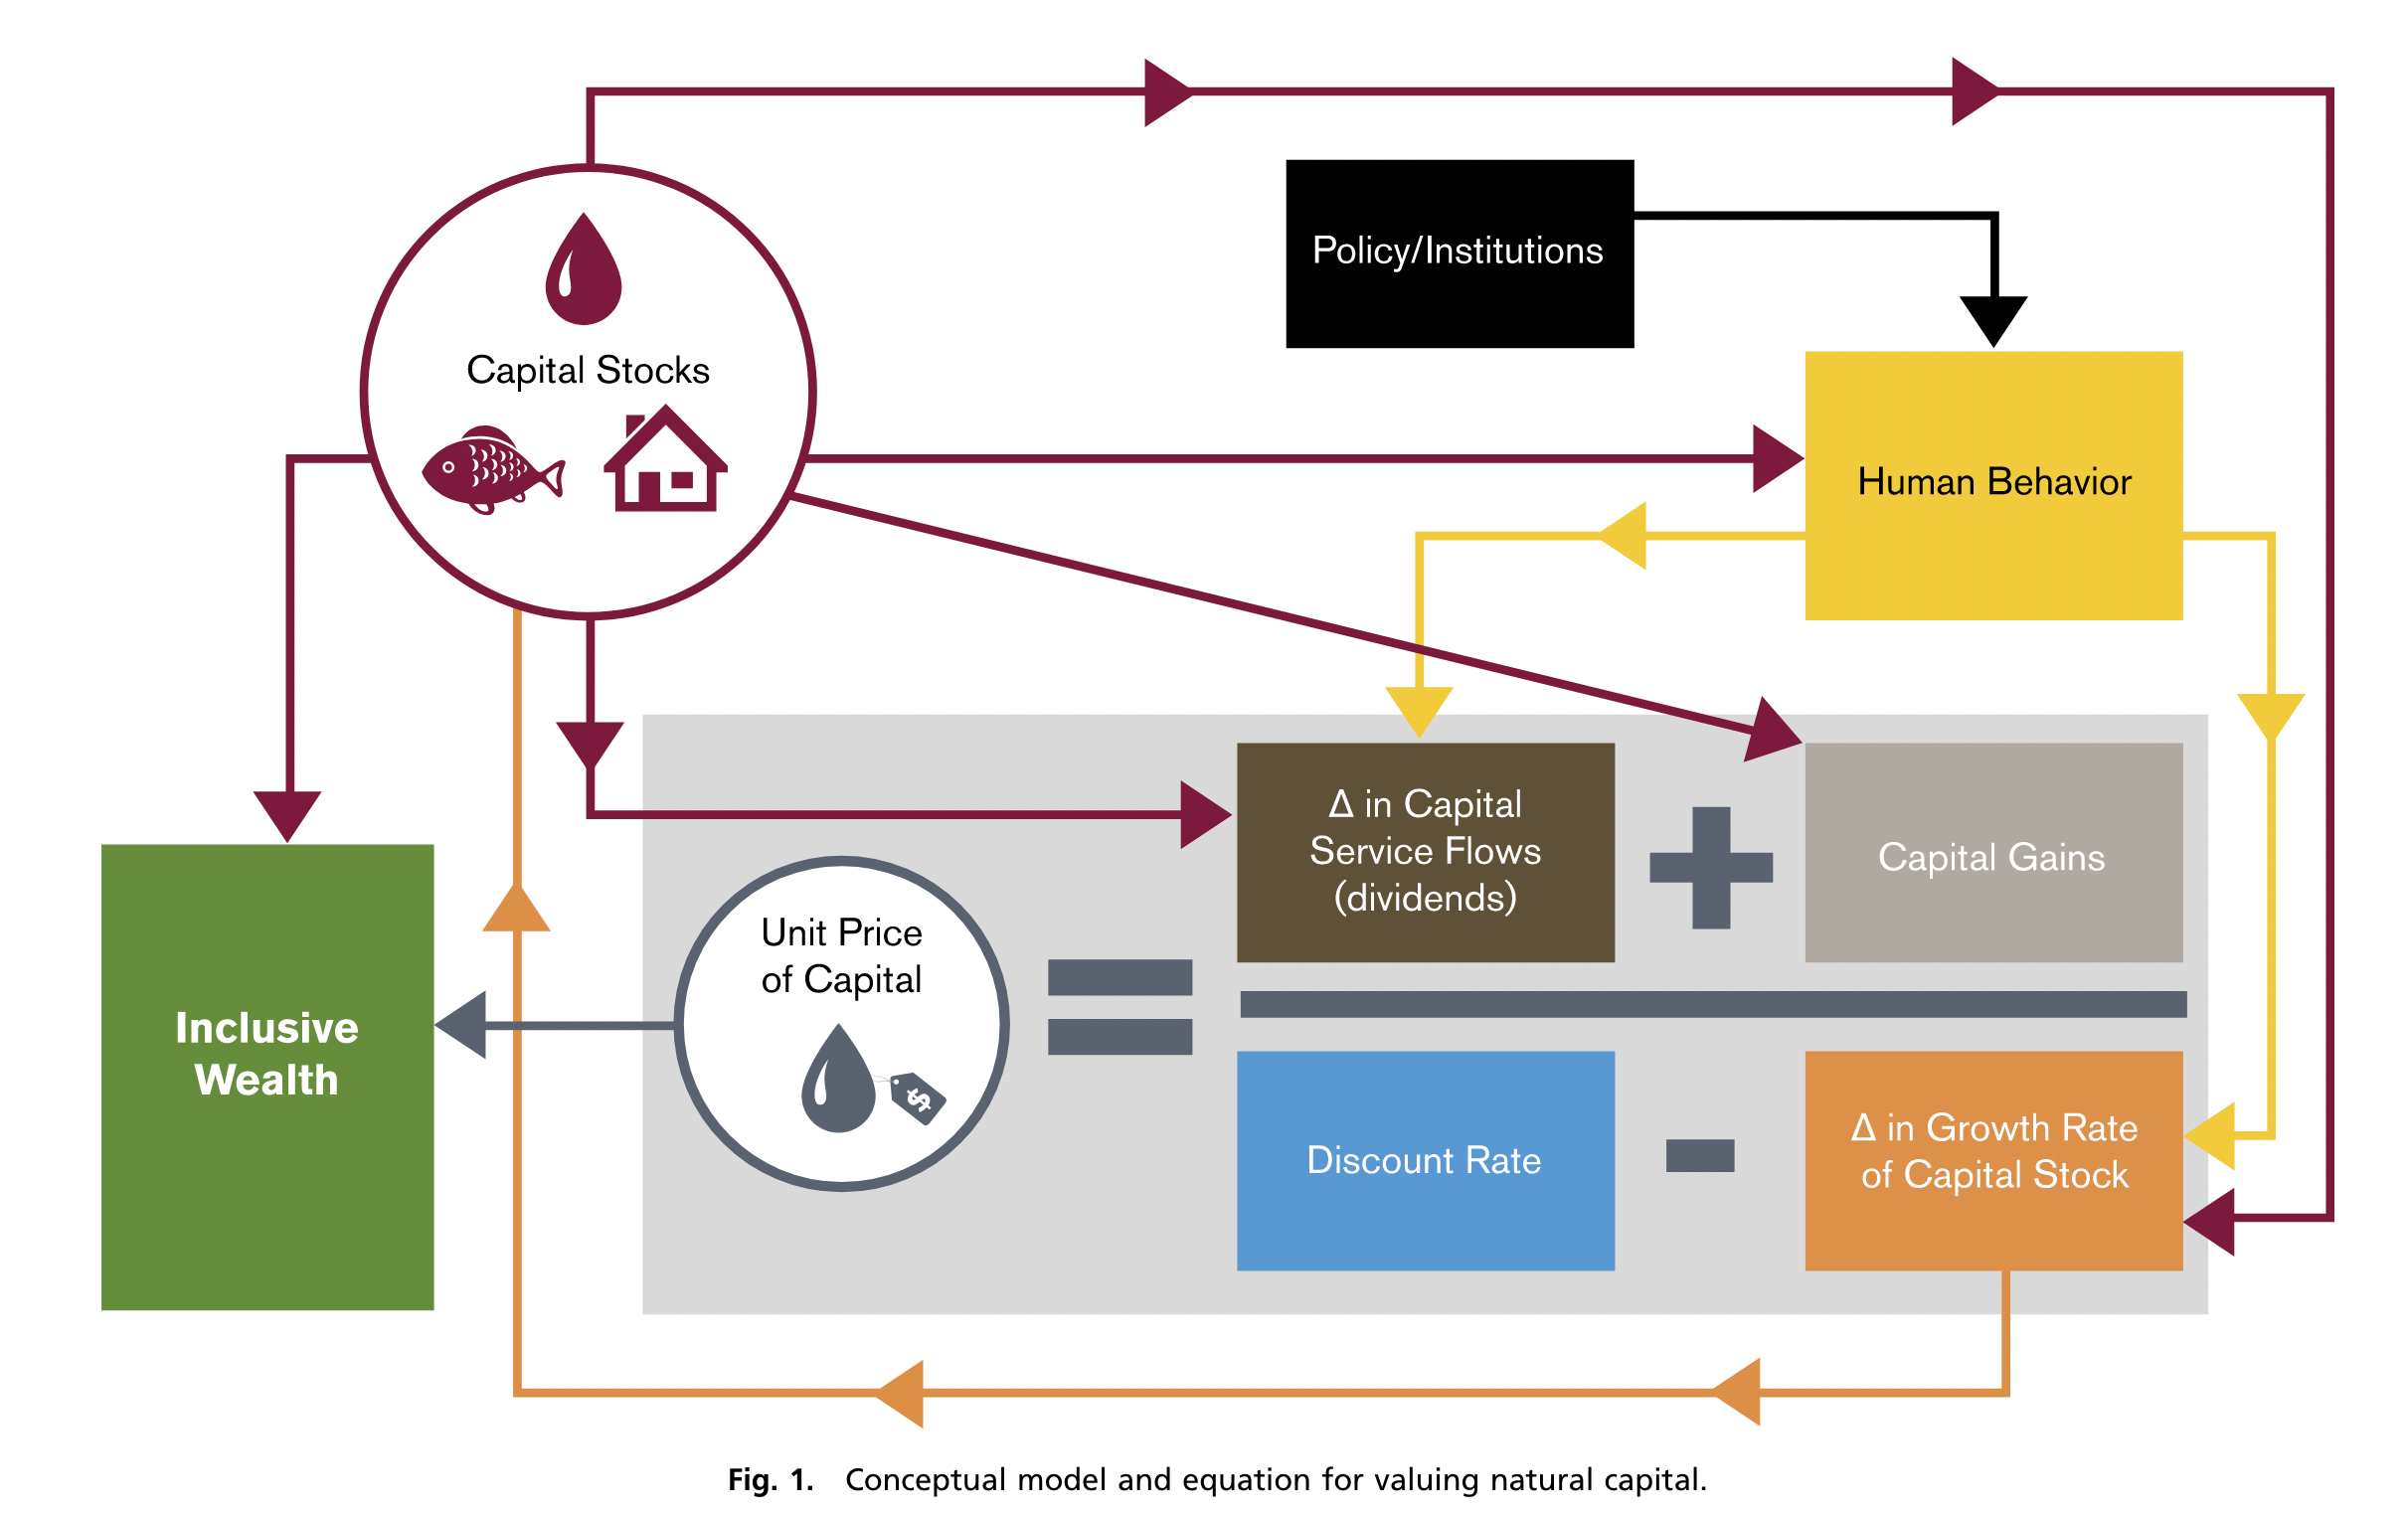
\includegraphics[width=14cm]{Screen Shot 2023-02-20 at 10.06.29 AM.png}
    \caption{equation as figure}
    \label{price_fig}
\end{figure}


We've now got one-ish unknown, which is the capital price $\lambda(s)$. The capital price $\lambda(s)$ is a function of its own derivative $\dot \lambda$. It is now possible to solve for the capital price $\lambda(s)$.\\

CAPn, the package Eli wrote, allows us to solve for the capital price $\lambda(s)$ despite it being a function of its own derivative. The key link is recognizing that \ref{cap_price} is just a function of $s$. We know that any function can be approximated by a polynomial. Traditionally, we use a polynomial called a Taylor approximation to approximate a function. The CAPn package uses a chebychev polynomial to approximate \ref{cap_price}.\\


CAPn solves for the capital price by first approximating the value function \ref{value_2} with a chebychev polynomial $\Phi(s)$

\begin{align}
    V(S(t)) & = \frac{W(s, x(s)) + \lambda(s) \dot s}{\delta}\\
    & \approx \Phi(s) \\
    & = \mathbf{\beta}F(s)\\
    & = \beta_0 + \beta_1 s + \beta_2 s^2 + \beta_3 s^3 + ...
    \label{chebychev_1}
\end{align}

Once we have $\Phi(s)$ from the CAPn package, we appeal to the definition of capital price being defined as marginal value \textit{once more} to get 

\begin{align}
    \lambda(S(t)) & = \frac{\partial }{\partial s} V(S(t))\\
    & \approx \frac{\partial}{\partial s} \Phi(s) \\
    & =\beta F'(s)
\end{align}

and have found our capital price $\lambda(S)$. \\


\subsection{Change in value of a stock}
It's important to recognize that price is a function of the stock size! If you have a ton of a good, it's not that valuable (ie the price will be lower). \textbf{Price is a measure of scarcity.} If that good gets scare, the price will increase. Example: eggs in 2023, because there has been an avian flu, there are fewer eggs and the price has gone up. \\

The relationship of stock and price is typically non-linear (it's a convex function). Therefore, the change in value from stock level $s_1$ to $s_2$ is hard to calculate when you don't the price curve 
$$\Delta V \neq p_2 s_2 - p_1 s_1$$

A rule to approximate this is 
$$ \Delta V = \frac{1}{2} (p_2 + p_1) (s_2 - s_1) $$
Eli has a paper showing this is a fairly good rule. 

\begin{figure}[htp]
    \centering
    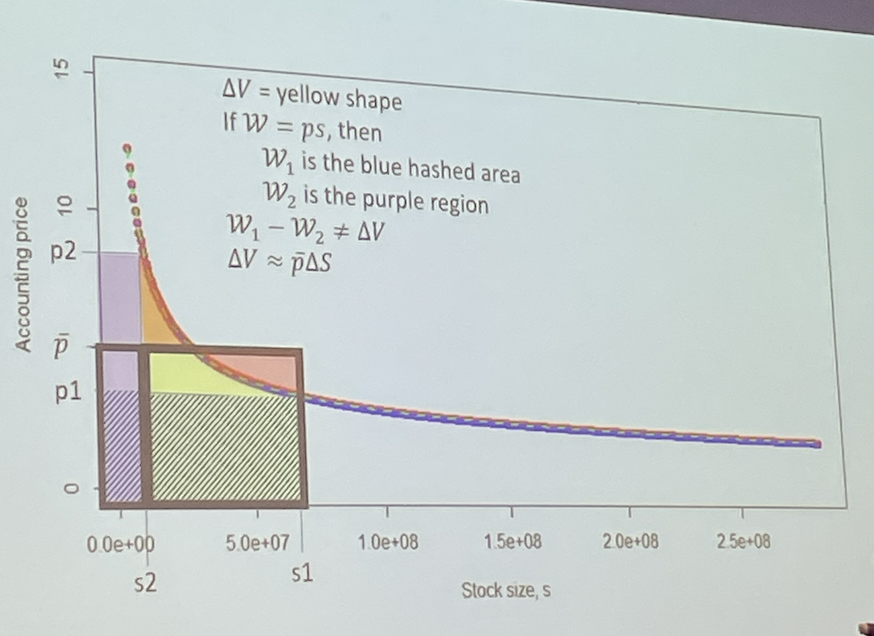
\includegraphics[width=14cm]{Screen Shot 2023-02-20 at 10.09.06 AM.png}
    \caption{price curve}
\end{figure}

\section{Substitutes vs Complements}
Not all natural capital stocks will be substitutes. Sometimes two natural capital stocks will be complements, one's existence aids the other's. 




\end{document}